\hypertarget{group__inv__park}{}\section{Vector Inverse Park transform}
\label{group__inv__park}\index{Vector Inverse Park transform@{Vector Inverse Park transform}}
Collaboration diagram for Vector Inverse Park transform\+:
\nopagebreak
\begin{figure}[H]
\begin{center}
\leavevmode
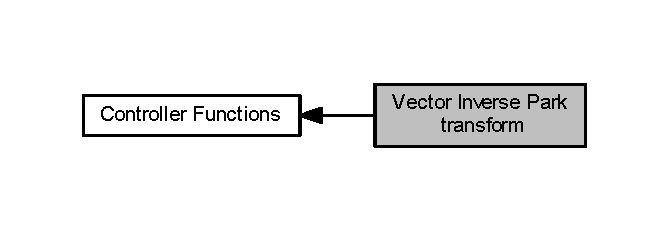
\includegraphics[width=321pt]{group__inv__park}
\end{center}
\end{figure}


\subsection{Detailed Description}
Inverse Park transform converts the input flux and torque components to two-\/coordinate vector.

The function operates on a single sample of data and each call to the function returns the processed output. The library provides separate functions for Q31 and floating-\/point data types. \begin{DoxyParagraph}{Algorithm}
 where {\ttfamily p\+Ialpha} and {\ttfamily p\+Ibeta} are the stator vector components, {\ttfamily Id} and {\ttfamily Iq} are rotor vector components and {\ttfamily cos\+Val} and {\ttfamily sin\+Val} are the cosine and sine values of theta (rotor flux position). 
\end{DoxyParagraph}
\begin{DoxyParagraph}{Fixed-\/\+Point Behavior}
Care must be taken when using the Q31 version of the Park transform. In particular, the overflow and saturation behavior of the accumulator used must be considered. Refer to the function specific documentation below for usage guidelines. 
\end{DoxyParagraph}
